%%%%%%%%%%%%%%%%%%%%%%%%%%%%%%%%%%%%%%%%%%%%%%%%%%%%%%%%%%%%%%%%%%%%%%%%%%%%%%%%
%2345678901234567890123456789012345678901234567890123456789012345678901234567890
%        1         2         3         4         5         6         7         8

\documentclass[letterpaper, 11pt, journal, final]{IEEEtran}

% \IEEEoverridecommandlockouts                              % This command is only
                                                          % needed if you want to
                                                          % use the \thanks command
% \overrideIEEEmargins
% See the \addtolength command later in the file to balance the column lengths
% on the last page of the document

\usepackage{hyperref}
\hypersetup{
    colorlinks=true,
    linkcolor=blue,
    filecolor=magenta,      
    urlcolor=cyan,
    citecolor=blue
}

\bibliographystyle{unsrt}
\usepackage[superscript,biblabel]{cite}

\usepackage{graphicx}
\graphicspath{ {./images/} }

\usepackage{mathtools}
\DeclarePairedDelimiter\ceil{\lceil}{\rceil}
\DeclarePairedDelimiter\floor{\lfloor}{\rfloor}

\usepackage{amsmath}
\DeclareMathOperator*{\argmax}{argmax\,}
\DeclareMathOperator*{\argmin}{argmin\,}
\DeclareMathOperator*{\dict}{dict[a]\!}

\usepackage{float}

\usepackage[table]{xcolor}% http://ctan.org/pkg/xcolor

\usepackage{pgfplots}
\usepackage{listings}

\usepackage{amsfonts}
% \renewcommand*\descriptionlabel[1]{\hspace\leftmargin$#1$}

% The following packages can be found on http:\\www.ctan.org
%\usepackage{graphics} % for pdf, bitmapped graphics files
%\usepackage{epsfig} % for postscript graphics files
%\usepackage{mathptmx} % assumes new font selection scheme installed
%\usepackage{times} % assumes new font selection scheme installed
%\usepackage{amsmath} % assumes amsmath package installed
%\usepackage{amssymb}  % assumes amsmath package installed

\title{\LARGE \bf
Modelling Markov Decision Processes for Solving Pac-Man in a Non-Deterministic, Fully Observable Environment with Random Agents
}

% \setlength{\footskip}{20pt}

\author{Oluwafemi Oladipo}

% \rfoot{Page \thepage \hspace{1pt} of \pageref{LastPage}}

\begin{document}
\maketitle

% \tableofcontents

% \newpage

% \begin{abstract}
% This is a review of journals in the area of using Artificial Intelligence for Intrusion Detection and Prevention Systems. The journals have discussed the milestones that have been achieved in the area of network security particularly intrusion detection. They has also highlighted several Machine Learning algorithms that can be applied in this area to improve the IDS systems.
% Four articles have been reviewed titled as follows: -
% \end{abstract}

\section{Introduction}
This paper evaluates the effectiveness of solving Pac-Man using solely a Markov Decision Process (MDP). Meaning Pac-Man's decision to make a move at any point (choose a policy) in time is solely determined by the best policy suggested by the MDP. This paper implements the MDP in python (version 2.7), with all the logic pertaining to the MDP contained within a single class MDPAgent. Finally, a few helper classes are also created to help represent the environment while keeping the code clean\cite{martin2009clean} and DRY\cite{dryCode}.

\section{Environment}
Representing the environment was the first priority in order to implement an efficient MDP solver. I achieved this using three classes, a Grid Class, a Point Class and a States Class.

\subsection{States Class}
Enum of states for the point class, being: empty, pacman, food, capsule, ghost\_hostile, ghost\_edible, ghost\_neighbour. Going forwards all three ghost states will be referred to as ghost for simplicity. However, whenever a specific sub category needs to be referenced its full name will be used.

\subsection{Grid Class}
Contains a representation of the 2D world Pac-Man operates in.

\subsection{Point Class}
Represents a single position on the grid. Each point has a type representing it's state, a utility representing it's current utility value, and a dynamic reward.

\section{Markov Decision Process}
The MDP in this paper is modelled using the bellman update\cite{Bel} formula, because simultaneous nature of the standard bellman equation proves unwieldy to solve. The MDPAgent class has various methods that help achieve different all the calculations, figure \ref{fig:mdpgent} depicts the hierarchy of calls.

\begin{figure}[ht]
    \centering
    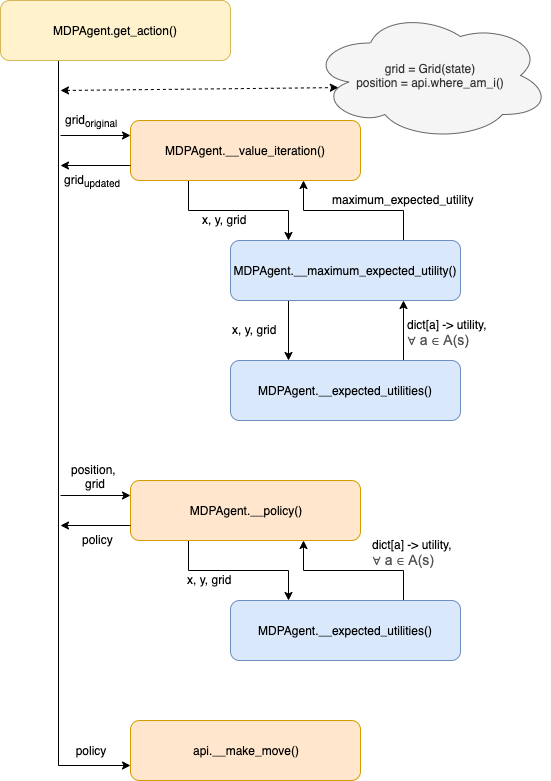
\includegraphics[width=8cm]{MDPAgent.png}
    \caption{\(MDPAgent.get\_action()\) call stack.}
    \label{fig:mdpgent}
\end{figure}

\begin{itemize}
    \item \textbf{MDPAgent.get\_action()} - creates a new grid object from the current state, and finds pacman current position. Then uses this information to call subsequent methods, to; perform value iteration on the grid, and find the optimum policy on the updated grid from current position.
    \item \textbf{MDPAgent.\_\_value\_iteration()} - performs the value iteration algorithm\cite{Bel}. It also applies the bellman update formula at each point.
    \[U_{i+1}(s) \gets R(s) + \gamma \max_{a \epsilon A(s)}  \sum\limits_{s^\prime} P(s^\prime|s, a) U_i(s^\prime)\]
    The reward value \(R(s)\) is calculated in the Point class. With the remaining of the formula being calculated in MDPAgent.\_\_maximum\_expected\_utility().
    \item \textbf{MDPAgent.\_\_policy()} - Finds the optimum policy for the next move. Using the following formula:
    \[\pi_{i+1} = \argmax_{a \epsilon A(s)} \sum_{s^\prime} P(s^\prime | s, a)
    U(s^\prime)\]
    Policy however only performs the argmax operation, while MDPAgent.\_\_expected\_utilities()  performs the calculation to find the scaled probability of the utility of each next state.
    \item \textbf{MDPAgent.\_\_maximum\_expected\_utility()} - Calculates the maximum expected utility at a point by taking the maximum utility of its surrounding points. Using the following formula:
    \[\max_{a \epsilon A(s)}  \sum\limits_{s^\prime} P(s^\prime|s, a) U_i(s^\prime)\]
    However, only the max operation is performed here, the rest of the formula is performed in MDPAgent.\_\_expected\_utilities().
    \item \textbf{MDPAgent.\_\_expected\_utilities()} - Creates a dictionary mapping all possible policies to their respective utilities.
    \[ \dict_{a \epsilon A(s)} \gets \sum\limits_{s^\prime} P(s^\prime|s, a) U_i(s^\prime)\]
\end{itemize}

\section{Methodology \& Creativity}
\subsection{Code Implementation}
Various design choices have been made in order to make the code a readable, and flexible as possible. This subsection details a few of these decisions.
\subsubsection{Effective Use of Data Models}
The grid class makes effective use of three python data model methods, \_\_getitem\_\_, \_\_iter\_\_ and \_\_contains\_\_.

\textbf{\_\_getitem\_\_ }is used so that points on instances of the grid class can be indexed by:
\begin{lstlisting}[language=Python]
g = Grid() 
point = g[x,y]
\end{lstlisting}
As opposed to, defining a get method to be used as:
\begin{lstlisting}[language=Python]
g = Grid()
point = g.get(x,y)
\end{lstlisting}
In addition, with the absence of a \_\_setitem\_\_ method, this prevents inadvertent assigning values to points in the grid. Meaning that following is invalid
\begin{lstlisting}[language=Python]
g = Grid()
g[x,y] = N
\end{lstlisting}
Which would invalidate the data structure, as all coordinates should index an instance of the point class and not arbitrary values. Or worse defining, a set method to be used as:
\begin{lstlisting}[language=Python]
g = Grid()
g.set(x,y,N)
\end{lstlisting}
Which would in validate the data structure, and create a lengthy syntax to be remembered. Instead, points can be updated only using the syntax: 
\begin{lstlisting}[language=Python]
g = Grid()
g[x,y].utility = N
\end{lstlisting}

\textbf{\_\_iter\_\_} is used to iterate through the underlying coordinates, and points on the grid. In addition, this allows easy iteration through all points in the value iteration algorithm. While also making it easier to skip wall coordinates by omitting them in the grid.

\textbf{\_\_contains\_\_} is used to check if a coordinate is valid grid non-wall grid position.

\subsubsection{Adhering to PEP8}
The base project is written using primarily camel casing, however python standards (PEP8) dictates that snake casing should be used. In order to interface with the base project, while using snaking casing, a series of function were created that aliased all imported functions as their a snake cased variant. They were then called on the imports:
\begin{lstlisting}[language=Python]
snake_case(util)

snake_case(api)
\end{lstlisting}
Allowing the use of functions in the form:
\begin{lstlisting}[language=Python]
api.legal_actions(state)

util.manhattan_distance(xy1, xy2)
\end{lstlisting}
Then all the methods in MDPAgent claas were aliased as their camel case variant, using a decorator.
\begin{lstlisting}[language=Python]
@camel_case
class MDPAgent(Agent):
\end{lstlisting}
Allowing core methods to be defined as:
\begin{lstlisting}[language=Python]
def get_action(state):

def register_initial_state(state):
\end{lstlisting}


\subsection{Strategy}
Pac-Man makes his decisions using solely the output of the MDP model. However, adjusting parts of the input has shown to improve the performance (win rate) of Pac-Man overall. In addition, some optimisations have also been made in terms of implementation in order to bring down the running time of the algorithm.

\subsubsection{Dynamic Reward Shaping}
Reward shaping is process by a reward \(r(s)\), is altered in order to cause faster convergence or better performance\cite{RewardShaping}. The point class handles the reward calculation and does so by employing subclass of reward shaping, dynamic reward shaping. That is, it employs a formula in each state to the final resulting reward. In the code accompanying this paper, this is done in the reward @property field in the point class.
\[
R(s) =
\left\{
\begin{array}{ll}
      food, capsule & r(s) \cdot f_\phi \div f_\Delta \\
     ghost, empty, pacman & r(s) \cdot f_\Delta \\
\end{array} 
\right.
\]

The cell five states: food, capsules, ghost, pacman and empty. Each cell state has a default reward value \(r(s)\). For the purposes of calculations, the default reward values are in two classes \(+ve\) and \(-ve\) values. This paper assigns \(+ve\) default reward values to food \& capsules only, and \(-ve\) default reward values to everything else (ghosts, pacman and empty cells). The goal is then to make the resulting reward \(R(s)\), either more or less \(+ve\) or \(-ve\) compared to the original \(r(s)\).\\

\textbf{Positive Rewards}
\[R(s) = \frac{r(s) \cdot f_\phi}{f_\Delta}\]
where
\begin{description}
\item[s \(\in\) \{food, capsule\}]
\item
\end{description}
In the positive default reward value class (food \& capsules) the goal is for the values to become less positive the closer they are to ghosts and more positive the further they are away. To ensure this default reward \(r(s)\) is  divided by a value between 1 and e  (\(f_\Delta\)). Where again items closer to ghosts are divided by values closer to e, therefore when divided the resulting value is less positive and less favourable. In addition, there is a competing multiplier (\(f_\phi\)) that increases foods reward value when there is less food available. The goal here is make Pac-Man seek out food more aggressively near the end of the game when food items are few and sparse.\\

\begin{figure}[ht]
    \centering
    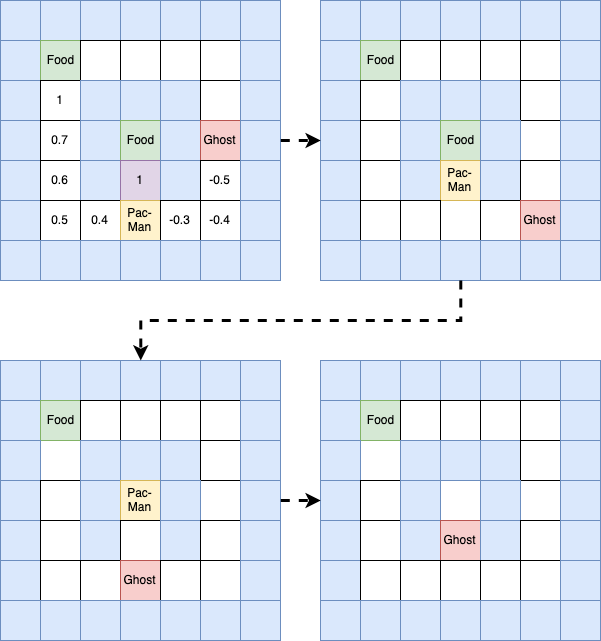
\includegraphics[width=8cm]{pre_manhattan.png}
    \caption{Diagram depicting optimum utility is north (purple), from the starting position. Then, how the resulting sequence of actions lead to Pac-Man's ultimate death.}
    \label{fig:pre_manhattan}
\end{figure}

Figure \ref{fig:pre_manhattan} shows how scaling the reward value food items can change optimum policy for the better. In this case, if Pac-Man goes directly north as suggest by the optimum policy (purple) he will often die in the sequence of events the figure shows. However, by employing the scaling technique, considering distance to ghosts, Pac-Man's optimum policy changes as shown in figure \ref{fig:post_manhattan}. In this scenario, if Pac-Man later goes for the food in the centre he'll survive as the game would have ended. The high level reasoning for this is that places nearer to a ghost are more risky, however when there are fewer pieces remaining the risk is decreased as Pac-Man should hopefully complete the game before being eaten.\\

\begin{figure}[ht]
    \centering
    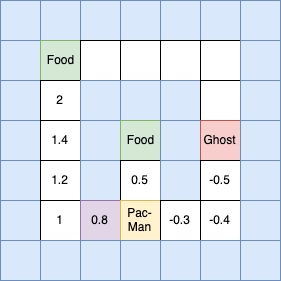
\includegraphics[width=4cm]{post_manhattan.png}
    \caption{Diagram depicting optimum policy (purple), is now east.}
    \label{fig:post_manhattan}
\end{figure}

\textbf{Negative Rewards}
\[R(s) = r(s) \cdot f_\Delta \]
where
\begin{description}
\item[s \(\in\) \{empty, ghost, pacman\}]
\item
\end{description}

The default reward of an empty cell is -0.04. However if this cell is near a ghost, then Pac-Man should avoid this cell more than an empty cell far away from any ghosts. In this case, the value needs to be more negative the closer it is to a ghost and less negative the further away. In order to achieve this the default reward is multiplied by a scalar between 1 and \(e\) \((f_\Delta)\), with empty cells closer to a ghost being multiplied by values closer to e. Hence making them more negative and less favourable. Likewise, the same happens for all other default rewards in the \(-ve\) value class.\\

\textbf{Peaking inside the functions}\\\\
Each function \(f_\Delta\) and \(f_\phi\) rely on a constant \(C\) derived from the environment. They then model the environment by raising \(e\) to the power of \(C\) (\(e^C\)).

\[f_\Delta= e^{\frac{D - d}{D}}\]
where:
\begin{description}
\item[D] is maximum manhattan distance of two points on grid
\item[d] is minimum manhattan distance between point and any ghost
\end{description}
Starting with the fraction, the top part \(D - d\) will give values between 0 and \(D\). Therefore when divided by \(D\) the result will between 0 and 1. Tending to 0 the closer d is to D (the point is far from any ghost), tending to D when d is nearly 0 (the point is adjacent to a ghost). Resulting in \(f_\Delta\) tending to e when point is far from any ghost, and tending to 1 when the point is adjacent to a ghost.


\[f_\phi= e^{\frac{s}{S}}\]
where:
\begin{description}
\item[S] is the total number of spaces on the grid
\item[s] is the numbers of spaces that are empty
\item
\end{description}

\(\frac{s}{S}\) will range between 0 and 1 inclusive. Tending to 0 when when s is close to 0 (there is a lot of food remaining), tending to 1 when s is close to S (there is hardly any food remaining). \(f_\phi\) will range between 1 and \(e\), tending to 1 when there is a lot of food remaining and tending to \(e\) when there is hardly any food remaining.

\subsubsection{Variable Discount Factor}
\[\gamma(x) = A + \frac{K - A}{1 + e^{-B(x-M)}}\]
where:
\begin{description}
\item[K] is the upper asymptote (1)
\item[A] is the lower asymptote (0.5)
\item[B] is the growth rate from left to right (-0.1)
\item[M] is the midpoint of the growth area (5)
\item[\(x\)] is the number of remaining food + capsules
\item
\end{description}

In this environment the game ends either when, all the pieces are eaten or Pac-Man is eaten by a ghost. With the favourable of the two states being that all pieces are eaten. Therefore all pieces being eaten can be conceptualised as the goal state. Assuming this, initially the grid has a near infinite horizon\cite{russell2016artificial}, so additive rewards will be inadmissible and discounted rewards are required. However the closer we are to the end (the fewer food pieces remaining) the more definite the route to the goal state. At the extreme, when there is one food piece remaining meaning we can use actual additive rewards. As such gamma has been modelled to reflect this. Varying between 0.6 and 1, increasing to values closer to one with fewer food pieces remaining. In order to model this shape Richard's Curve\cite{richardsCurve}, a flexible/malleable sigmoid curve has been used.

\subsubsection{Terminal States}
Since in this environment the game ends either when, all the pieces are eaten or Pac-Man is eaten by a ghost. The ghosts are therefore also an end state, however an undesirable one. So similar to increasing gamma to more resemble additive rewards for fewer and fewer food items. Ghosts are treated as terminal states, meaning there utility values never change. This has the effect of creating a well around them, ensuring the surrounding values are negative. In addition it ensures the the ghosts utility value doesn't become positive when surrounded by only food. \cite{Bel}.


\subsubsection{Convergence}
\[\lim_{iteration} = 2 * \ceil*{\sqrt{height * width}}\]
The number of iterations used to converge the utility values has a big affect on the success of the MDP. However, although generally increasing the number of iterations leads to higher success the running time of the program also increases and very quickly becomes unwieldy. In addition, through testing larger boards require more iterations. This is because, with more points on the board values have a further distance to propagate to.

\subsubsection{Hyper-Parameters}
To increase the ability for the utility values to accurately model the environment, ghost neighbours were introduced. These points have a negative default reward value (\(r(s) \in \mathbb{R}^-\)), which is less than that of an empty space. This was model by setting a maximum manhattan distance (radius) around any ghosts and point within were deemed ghost neighbours, except if they were walls or other ghosts. In addition, as ghosts move twice as fast as Pac-Man when they are edible the could become hostile again and eat Pac-Man quickly. However, to avoid this Pac-Man avoids ghosts when their remaining timer is less than a set value.

\section{Results}
To come up with the final version of MDPAgent, various design decisions had to be made such as; whether or not to use a variable discount factor, whether or not to use terminal states and which states should they be, and how to design the dynamic reward shaping functions, all of this in addition to initialising various hyper-parameters. All of which will be discussed in this section, with statistical evidence to back up decisions made. All experiments were repeated 10 times, with 10 iterations in each run. The statically relevant stat, used is then the average of all 100  iterations. For reference hence forth performance will, will refer to as the win percentage out of 100 iterations. Finally, most experiments have been conducted on both the smallGrid and mediumClassic layouts, however the grid/s used are always stated.

\subsection{Dynamic Reward Shaping}
To test the effect of including dynamic reward shaping, the first step was to test the condition that inspired it's creation. As detailed in methodology, figure \ref{fig:pre_manhattan} shows the starting position to which a high proportion of losses on the small grid were attributed to. Therefore a new starting layout was created in the this configuration which will be named smallGridCustom.

\begin{table}[h!]
\centering
\caption{Dynamic Reward Shaping on smallGridCustom}
\begin{tabular}{ c || c } 
 \hline
  Dynamic Reward & Win Rate (\%) \\
  \cline{2-2}
  Shaping & smallGridCustom \\
 \hline
 \cellcolor{blue!18}True & \cellcolor{blue!18}43 \\ [0.5ex]
 False & 25\\ [0.5ex]
 \hline
\end{tabular}
\end{table}

This demonstrated dynamic reward shaping works in the niche that inspired it, however testing what was then required was to show whether this performance increase continues in other situations.

\begin{table}[h!]
\centering
\caption{Dynamic Reward Shaping Test}
\begin{tabular}{c || c | c}
    \hline
    Dynamic Reward  & \multicolumn{2}{c}{Win Rate (\%)}\\
        \cline{2-3}
        Shaping & smallGrid & mediumClassic\\
    \hline
    \cellcolor{blue!18}True & \cellcolor{blue!18}57 & \cellcolor{blue!18}38 \\ [0.5ex]
    False & 41 & 18\\ [0.5ex]
    \hline
\end{tabular}
\end{table}


This demonstrates the general usefulness of dynamic reward shaping and that they increased overall performance. This method was therefore used in the final model.

\subsection{Variable Discount Factor}
A range of discount factor were tested used on both grids, from 0.l to 1.

% \begin{table}[h!]
% \centering
% \caption{Static Discount Factor Test}
% \begin{tabular}{c || c | c} 
%  \hline
%  Discount & \multicolumn{2}{c}{Win Rate (\%)}\\
%         \cline{2-3}
%         Factor & smallGrid & mediumClassic\\
%  \hline
%  0.1 & 0 & 0 \\ [0.5ex]
%  0.2 & 3 & 0  \\ [0.5ex]
%  0.3 & 2 & 0  \\ [0.5ex]
%  0.4 & 3 & 2 \\ [0.5ex]
%  0.5 & 40 & 28 \\ [0.5ex] 
%  0.6 & 51 & \cellcolor{blue!18}42 \\ [0.5ex] 
%  0.7 & \cellcolor{blue!18}57 & 38 \\ [0.5ex] 
%  0.8 & 55 & 37 \\ [0.5ex] 
%  0.9 & 56 & 37 \\ [0.5ex] 
%  \hline
% \end{tabular}
% \end{table}

\begin{center}
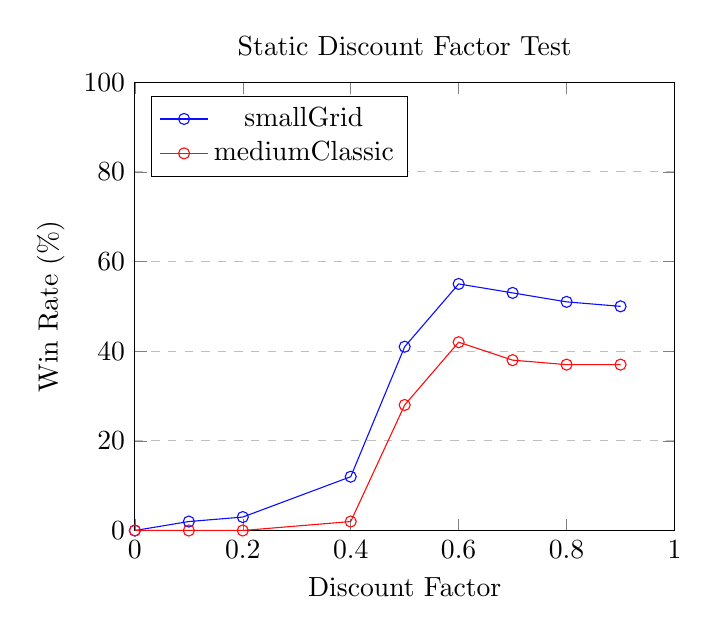
\begin{tikzpicture}
\begin{axis}[
    title={Static Discount Factor Test},
    xlabel={Discount Factor},
    ylabel={Win Rate (\%)},
    xmin=0, xmax=1,
    ymin=0, ymax=100,
    % xtick={0,0.2,0.4,0.6,0.8,1},
    % ytick={0,20,40,60,80,100},
    legend pos=north west,
    ymajorgrids=true,
    grid style=dashed,
]

\addplot[color=blue!95,mark=o]
    coordinates {
    (0,0)(0.1,2)(0.2,3)(0.4,12)(0.5,41)(0.6,55)(0.7,53)(0.8,51)(0.9,50)
    };
    \addlegendentry{smallGrid}

\addplot[color=red!95,mark=o]
    coordinates {
    (0,0)(0.1,0)(0.2,0)(0.4,2)(0.5,28)(0.6,42)(0.7,38)(0.8,37)(0.9,37)
    };
    \addlegendentry{mediumClassic}
\end{axis}
\end{tikzpicture}
\end{center}


The results showed a discount factor in the open interval (0.5, 1) were the most successful. However, smallGrid and mediumClassic had different peaks. This was due to them starting at different distances away from their end state (see section IV.B Variable Discount Factor). As such a final setting varying gamma, dependant on the remaining number of pieces, was tested. Always setting the upper bound to 1 (additive rewards), and tested different lower bounds within the optimal range.

% \begin{table}[h!]
% \centering
% \caption{Variable Discount Factor Test}
% \begin{tabular}{c || c| c} 
%  \hline
%  Discount Factor & \multicolumn{2}{c}{Win Rate (\%)}\\
%         \cline{2-3}
%         Interval & smallGrid & mediumClassic\\ 
%  \hline
%  (0.9, 1) & 58 & 37 \\ [0.5ex]
%  (0.8, 1) & 58 & 38\\ [0.5ex]
%  (0.7, 1) & 59 & 40\\ [0.5ex]
%  \cellcolor{blue!18}(0.6, 1) & \cellcolor{blue!18}61 & \cellcolor{blue!18}42\\ [0.5ex]
%  (0.5, 1) & 60 & 39\\ [0.5ex]
%  \hline
% \end{tabular}
% \end{table}

\begin{center}
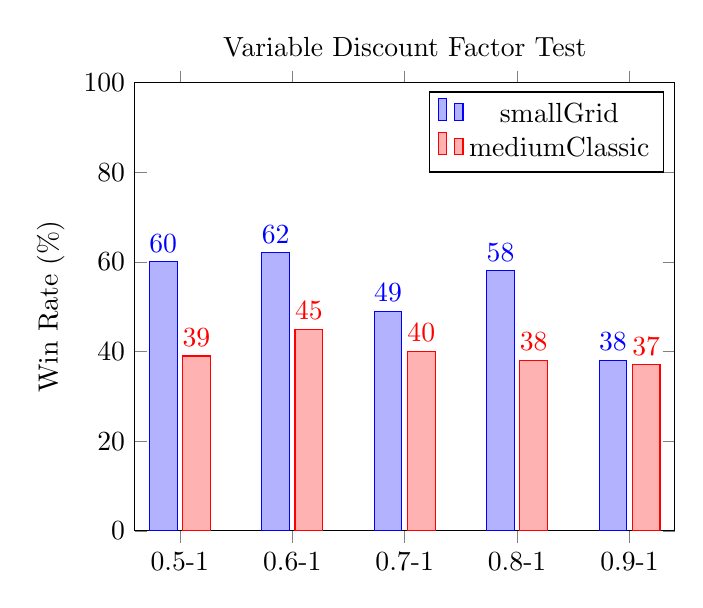
\begin{tikzpicture}
\begin{axis}[
    title={Variable Discount Factor Test},
    ybar,
    ymin=0, ymax=100,
    ylabel={Win Rate (\%)},
    symbolic x coords={0.5-1, 0.6-1, 0.7-1, 0.8-1, 0.9-1},
    xtick=data,
    nodes near coords,
]
\addplot coordinates {(0.5-1,60) (0.6-1,62) (0.7-1,49) (0.8-1,58) (0.9-1,38)};
\addplot coordinates {(0.5-1,39) (0.6-1,45) (0.7-1,40) (0.8-1,38) (0.9-1,37)};
\legend{smallGrid, mediumClassic}
\end{axis}
\end{tikzpicture}
\end{center}

The results showed varying gamma, always lead to higher performance than any static gamma value. How it also showed varying gamma in the open interval (0.6, 1) was the most optimal.

\subsection{Terminal States}
The aim of using terminal states was to reduce running time, while not affecting performance.

\begin{table}[h!]
\centering
\caption{Terminal States Test}
\begin{tabular}{c || c| c} 
 \hline
 Terminal & \multicolumn{2}{c}{Win Rate (\%)}\\
        \cline{2-3}
        States & smallGrid & mediumClassic\\
 \hline
 none & 55 & 34 \\ [0.5ex]
 ghosts only & \cellcolor{blue!18}57 & \cellcolor{blue!18}39 \\ [0.5ex]
 food only & 35 & 18\\ [0.5ex]
 ghosts \& food & 40 & 22\\ [0.5ex]
 \hline
\end{tabular}
\end{table}

\begin{table}[h!]
\centering
\caption{Terminal States (Running Time) Test}
\begin{tabular}{c || c| c} 
 \hline
 Terminal & \multicolumn{2}{c}{Running Time (seconds)}\\
        \cline{2-3}
        States & smallGrid & mediumClassic\\
 \hline
 none & 3 & 320\\ [0.5ex]
 ghosts only & 3 & 270 \\ [0.5ex]
 food only & 2 & 250\\ [0.5ex]
 ghosts \& food & \cellcolor{blue!18}1 & \cellcolor{blue!18}200\\ [0.5ex]
 \hline
\end{tabular}
\end{table}

% \begin{center}
% \begin{tikzpicture}
% \begin{axis}[
%     title={Variable Discount Factor on smallGrid},
%     ybar,
%     ymin=0, ymax=100,
%     ylabel={Win Rate (\%)},
%     symbolic x coords={0.5-1, 0.6-1, 0.7-1, 0.8-1, 0.9-1},
%     xtick=data,
%     nodes near coords,
% ]
% % win rate
% \addplot coordinates {(0.5-1,7) (0.6-1,9) (0.7-1,4) (0.8-1,32) (0.9-1,30)};
% \addplot coordinates {(0.5-1,7)};
% \legend{Win Rate, Running Time}
% \end{axis}

% \pgfplotsset{every axis y label/.append style={rotate=180,yshift=9cm}}

% \begin{axis}[
%     ybar,
%     hide x axis,
%     ymin=0, ymax=400,
%     axis y line*=right,
%     symbolic x coords={0.5-1, 0.6-1, 0.7-1, 0.8-1, 0.9-1},
%     nodes near coords,
%     ylabel={Running Time (secs)}
% ]
% % running time
% \addplot coordinates {};
% \addplot coordinates {(0.5-1,300) (0.6-1,250) (0.7-1,270) (0.8-1,200) (0.9-1,200)};
% \end{axis}

% \end{tikzpicture}
% \end{center}

% \begin{center}
% \begin{tikzpicture}
% \begin{axis}[
%     title={Variable Discount Factor on mediumClassic},
%     ybar,
%     ymin=0, ymax=100,
%     ylabel={Win Rate (\%)},
%     symbolic x coords={0.5-1, 0.6-1, 0.7-1, 0.8-1, 0.9-1},
%     xtick=data,
%     nodes near coords,
% ]
% % win rate
% \addplot coordinates {(0.5-1,7) (0.6-1,9) (0.7-1,4) (0.8-1,32) (0.9-1,30)};
% \addplot coordinates {(0.5-1,7)};
% \legend{Win Rate, Running Time}
% \end{axis}

% \pgfplotsset{every axis y label/.append style={rotate=180,yshift=9cm}}

% \begin{axis}[
%     ybar,
%     hide x axis,
%     ymin=0, ymax=400,
%     axis y line*=right,
%     symbolic x coords={0.5-1, 0.6-1, 0.7-1, 0.8-1, 0.9-1},
%     nodes near coords,
%     ylabel={Running Time (secs)}
% ]
% % running time
% \addplot coordinates {};
% \addplot coordinates {(0.5-1,300) (0.6-1,250) (0.7-1,270) (0.8-1,200) (0.9-1,200)};
% \end{axis}

% \end{tikzpicture}
% \end{center}

The results showed using only ghosts as terminal states was the most productive, when considering both running time and performance. As this was the only setting to reduce running time, without affecting performance.


\subsection{Hyper-Parameters}
Two hyper-parameters (ghost radius, and ghost safe time) were tested, with varied values against both layouts in-order to find their respective optimal values.

\textbf{Ghost Radius} - is the manahattan distance around ghosts that Pac-Man should avoid. The results showed having settings on smallGrid and mediumClassic would be . most optimal, having the values 0 and 3 respectively.

\begin{table}[h!]
\centering
\caption{Table to test captions and labels}
\begin{tabular}{c || c| c} 
 \hline
Ghost & \multicolumn{2}{c}{Win Rate (\%)}\\
\cline{2-3}
Radius & smallGrid & mediumClassic\\
 \hline
 0 & \cellcolor{blue!18}55 & 25\\ [0.5ex]
 1 & 54 & 25\\ [0.5ex]
 2 & 34 & 38\\ [0.5ex]
 3 & 0 & \cellcolor{blue!18}42\\ [0.5ex]
 4 & 0 & 40\\ [0.5ex]
 5 & 0 & 20\\ [0.5ex]
 \hline 
\end{tabular}
\end{table}

\textbf{Ghost Safe Time} - is amount of time remaining, whereby edible ghosts should be consider as hostile as regular ghosts. This was only tested on the mediumClassic layout as smallGrid had no capsules, so ghosts could never become edible. The results showed a time of 3 was as optimal as anyway great time, therefore this was used in-order to keep the restiction low.

\begin{table}[h!]
\centering
\caption{Table to test captions and labels}
\begin{tabular}{c || c} 
 \hline
Ghost Safe & {Win Rate (\%)}\\
\cline{2-2}
Time & mediumClassic\\
 \hline
 0 & 25 \\ [0.5ex]
 1 & 25 \\ [0.5ex]
 2 & 24 \\ [0.5ex]
 \cellcolor{blue!18}3 & \cellcolor{blue!18}41 \\ [0.5ex]
 4 & 40 \\ [0.5ex]
 5 & 41 \\ [0.5ex]
 \hline
\end{tabular}
\end{table}

\section{Conclusion}
The the non-deterministic fact about the environment played a big factor in the final performance, as testing with the same final configuration but turning of the non-deterministic effect yielded a performance of 100\% and 85\% in smallGrid and mediumClassic respectively. Where as with the non-deterministic effect turned on yielded a performance of 60\& and 40\% on smallGrid and mediumClassic respectively. Overall, this demonstrates that an MDP model can accurately select the best policy in a Non-Deterministic, Fully Observable Environment with Random Agents. However, further research how can be done to see if combining this with ad-hoc heuristics such as avoiding ghosts at the last minute, and planning the shortest path to a food item will further increase the performance.

% \newpage
\bibliographystyle{plain}
\bibliography{references}

\end{document}
